\documentclass[a4paper]{article}

  \usepackage{fullpage} % Package to use full page
  \usepackage{parskip} % Package to tweak paragraph skipping
  \usepackage{tikz} % Package for drawing
  \usepackage{amsmath}
  \usepackage{siunitx} % Package for scientific units
  \usepackage{amsfonts}
  \usepackage{amssymb}
  \usepackage{hyperref}
  \usepackage[utf8]{inputenc}
  \usepackage[english]{babel}
  \usepackage{multicol}
  \usepackage{graphicx} % Package for including images
  \graphicspath{ {./images/} }
  
  \newcommand\tab[1][0.5cm]{\hspace*{#1}}
  
  \title{Assignment 3}
  \author{Adrian Darian}
  \date{9/18/2020}
  
  \begin{document}
  
\maketitle
  
\section*{Chapter 3}
\begin{itemize}
	\item[7] In the circuits in Fig. P3.7 (a)-(d), find the equivalent resistance seen by the source and the power delivered by the source. \\
	      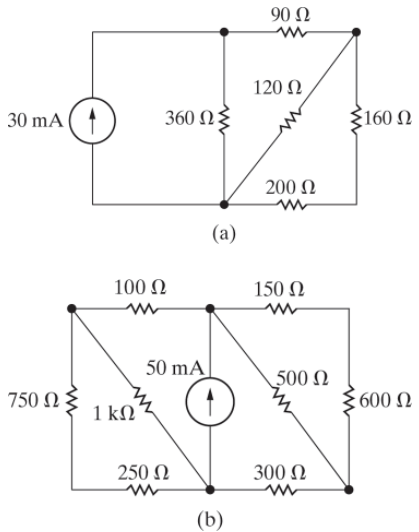
\includegraphics[scale=0.5]{3-7-a-b.png} \\ 
	      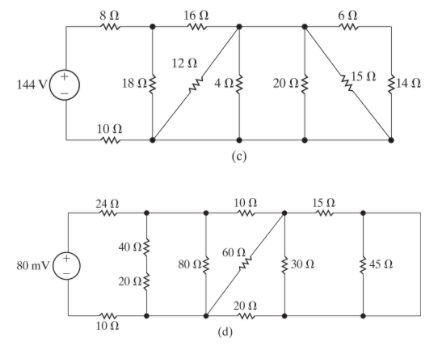
\includegraphics[scale=0.5]{3-7-c-d.png} \\ 
	      \begin{itemize}
	      	\item[a)] Resistance = $360 || ((200 + 160) || 120 + (200 + 160) || 120) = 120 Ohm$ \\
	      	      Power Delivered = $120(30)^2 = 108 mW$
	      	\item[b)] Resistance = $((250 + 750) || 1000) + 100 || ((600 + 150) || 500 + (600 + 150) || 500) = 300 Ohm$ \\
	      	      Power Delivered = $300(50)^2 = 750 mW$ 
	      	\item[c)] Resistance = $8 + (18 || (16 + ((((6 + 14) || 15) || 20 || 4) || 12))) + 10 = 27 Ohm$ \\
	      	      Power Delivered = $\frac{(144)^2}{27} = 768 W$
	      	\item[d)] Resistance = $24 + (30 || 60 || 80) + (((15 || 30) + 20) || 60) = 6 Ohm$ \\
	      	      Power Delivered = $\frac{(144)^2}{27} = 106.67 uW$
	      \end{itemize}
	\item[10] 
	      \begin{itemize}
	      	\item[a)] Find an expression for the equivalent resistance of two resistors of value R in series. \\
	      	      $R_{eq} = R + R = 2R$ 
	      	\item[b)] Find an expresion for the quivalent resistance of n resistors of value R in series. \\
	      	      $R_{eq} = R + R + R + ... + R = nR$ 
	      	\item[c)] Using the results of (a), design a resistive network with an equivalent resistance of 3 kOhm using two resistors with the same value from Appendix H. \\
	      	      $R + R = 2R = 3000$ \\
	      	      $R = 1500 Ohm$
	      	\item[d)] Using the results of (b), design a resistive network with an equivalent resistance of 4 kOhm using a minimum number of identical resistors from Appendix H. \\
	      	      $nR = 4R = 4000$ \\
	      	      $R = 1000 Ohm$
	      \end{itemize} 
	\item[16]
	      \begin{itemize}
	      	\item[a)] The voltage divider in Fig. P3.16 (a) is loaded with the voltage divider shown in Fig. P3.16 (b); that is, a is connected to a', and b is connected to b'. Find $v_{o}$. \\
	      	      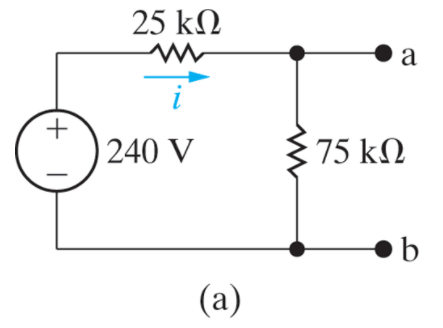
\includegraphics[scale=0.5]{3-16-a.png} \\  
	      	      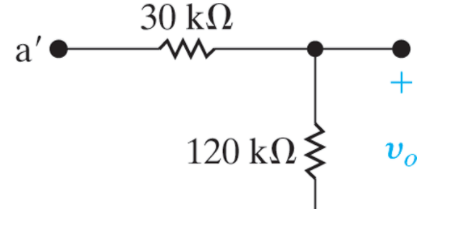
\includegraphics[scale=0.5]{3-16-b-1.png} \\ 
	      	      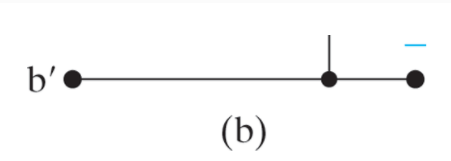
\includegraphics[scale=0.5]{3-16-b-2.png} \\ 
	      	      $75 kOhm || (120 kOhm + 30 kOhm) = 50 kOhm$ \\
	      	      $v_{o_{1}} = \frac{50 kOhm}{(75 kOhm)} * 240 V = 160 V$ \\
	      	      $v_{o} = \frac{120 kOhm}{150 kOhm} * v_{o_{i}} = 128 V$
	      	\item[b)] Now assume the voltage divider in Fig. P3.16 (b) is connected to the voltage divider in Fig. P3.16 (a) by means of a current-controlled voltage source as shown in Fig. P3.16 (c). Find $v_{o}$. \\
	      	      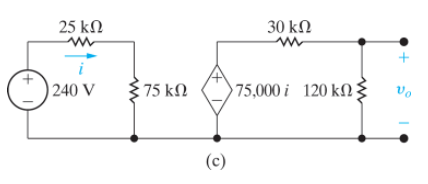
\includegraphics[scale=0.5]{3-16-c.png} \\  
	      	      $i = \frac{240 V}{100 kOhm} = 2.4 mA$ \\
	      	      $v_{o} = \frac{120}{150} * 75000i = 144 V$
	      	\item[c)] What effect does adding the dependent-voltage source have on the operation of the voltage divider that is connected to the 240 V source? \\
	      	      $v_{o_{1}} = 0.95 * 240 V = 180 V$
	      \end{itemize} 
	\item[19] For the current divider circuit in Fig. P3.19 calculate \\
	      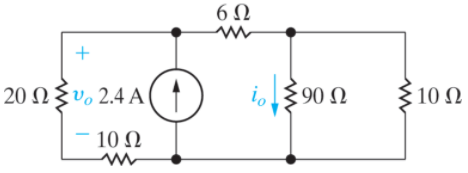
\includegraphics[scale=0.5]{3-19.png} \\  
	      \begin{itemize}
	      	\item[a)] $i_{o}$ and $v_{o}$. \\
	      	      \begin{tabular}{rcl}
	      	      	$R_{eq}$     & $=$ & $(10 + 20) || (6 + (90 || 10))$            \\
	      	      	             & $=$ & $10 Ohm$                                   \\
	      	      	$v_{2.4A}$   & $=$ & $10i$                                      \\
	      	      	             & $=$ & $2.4 * 10$                                 \\
	      	      	             & $=$ & $24 V$                                     \\
	      	      	$v_{o}$      & $=$ & $v_{20 Ohm}$                               \\
	      	      	             & $=$ & $(24) * \frac{10}{10 + 20}$                \\
	      	      	             & $=$ & $16 V$                                     \\
	      	      	$v_{90 Ohm}$ & $=$ & $24 * (\frac{(90 || 10)}{6 + (90 || 10)})$ \\
	      	      	             & $=$ & $14.4 V$                                   \\
	      	      	$i_{o}$      & $=$ & $\frac{v_{90 Ohm}}{90}$                    \\
	      	      	             & $=$ & $0.16 A$                                   \\
	      	      \end{tabular} 
	      	\item[b)] the power dissipated in the 6 Ohm resistor. \\
	      	      $P_{6 Ohm} = \frac{(v_{2.4A} - v_{90 Ohm})^2}{6} = \frac{(24 - 14.4)^2}{6} = 15.36 W$ 
	      	\item[c)] the power developed by the current source. \\
	      	      $P_{2.4A} = -(V_{2.4A})(i_{2.4A}) = -(2.4)(24) = -57.6 W$  
	      \end{itemize} 
	\item[31] Find $v_{o}$ in the circuit in Fig. P3.31 using voltage and/or current division. \\
	      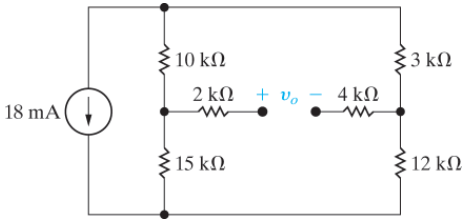
\includegraphics[scale=0.5]{3-31.png} \\  
	      \begin{tabular}{rcl}
	      	$i_{1}$   & $=$ & $\frac{-(18 mA)(3k + 12k)}{(3k + 12k) + (10k + 15k)}$ \\
	      	          & $=$ & $-6.75 mA$                                            \\
	      	$v_{15k}$ & $=$ & $i_{1}(15k)$                                          \\
	      	          & $=$ & $-101.25 V$                                           \\
	      	$i_{2}$   & $=$ & $i_{s} - i_{1}$                                       \\
	      	          & $=$ & $-11.25 mA$                                           \\
	      	$v_{12k}$ & $=$ & $(i_{12k})(12k)$                                      \\
	      	          & $=$ & $-135 V$                                              \\
	      	$v_{o}$   & $=$ & $v_{15 kOhm} - v_{12 kOhm}$                           \\
	      	          & $=$ & $33.75 V$                                             \\
	      \end{tabular} 
	\item[32] 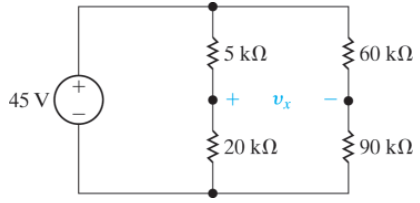
\includegraphics[scale=0.5]{3-32.png} \\ 
	      \begin{itemize}
	      	\item[a)] Find the voltage $v_{x}$ in the circuit in Fig. P3.32 using voltage and/or current division. \\
	      	      \begin{tabular}{rcl}
	      	      	$v_{20 kOhm}$ & $=$ & $45 * \frac{20 kOhm}{(20 kOhm + 5 kOhm)}$ \\
	      	      	             & $=$ & $36 V$                    \\
	      	      	$v_{90 kOhm}$     & $=$ & $45 * \frac{90 kOhm}{(90 kOhm + 60 kOhm)}$ \\
	      	      	             & $=$ & $27 V$                     \\
	      	      	$v_{x}$      & $=$ & $v_{20 kOhm} - v_{90 kOhm}$           \\
	      	      	             & $=$ & $9 V$                       \\
	      	      \end{tabular}  
	      	\item[b)] Replace the 45V source with a general voltage source equal to $V_{s}$. Assume $V_{s}$ is positive at the upper terminal. Find $v_{x}$ as a function of $V_{s}$. \\
	      	      \begin{tabular}{rcl}
	      	      	$v_{20k}$ & $=$ & $\frac{20k}{(20k + 5k)}(V_{s})$ \\
	      	      	         & $=$ & $0.8 V_{s}$                      \\
	      	      	$v_{90k}$ & $=$ & $\frac{90k}{(90k + 60k)}(V_{s})$ \\
	      	      	         & $=$ & $0.6 V_{s}$                      \\
	      	      	$v_{x}$  & $=$ & $v_{20k} - v_{90k}$             \\
	      	      	         & $=$ & $0.2 V_{s}$                   \\
	      	      \end{tabular}  
	      \end{itemize} 
\end{itemize}
    
\end{document}